\documentclass[12pt, a4paper]{book}

\usepackage[T1]{fontenc}
\usepackage[utf8]{inputenc}
\usepackage[charter, cal=cmcal]{mathdesign}
\usepackage[scaled=0.92]{helvet}
\usepackage{geometry}
\geometry{a4paper, top=30mm, bottom=30mm, inner=32mm, outer=25mm, marginparwidth=18mm}

\usepackage{amsmath, amsthm}
\usepackage[version=4]{mhchem}
\usepackage{graphicx}
\usepackage[dvipsnames,svgnames,table]{xcolor}
\usepackage{tikz}
\usetikzlibrary{arrows.meta, shapes.geometric, positioning, calc, backgrounds}
\usepackage{pgfplots}
\pgfplotsset{compat=1.18}
\usepackage{tcolorbox}
\tcbuselibrary{skins, breakable, theorems}
\usepackage{titlesec}
\usepackage{fancyhdr}
\usepackage{enumitem}
\usepackage{booktabs}
\usepackage{array}
\usepackage{multicol}
\usepackage{parskip}
\usepackage{siunitx}
\usepackage[colorlinks=true, linkcolor=BrickRed,
            urlcolor=NavyBlue, citecolor=ForestGreen]{hyperref}

\definecolor{JourneyColor}{HTML}{145A32}
\definecolor{ModuleColor}{HTML}{1E8449}
\definecolor{PuzzleColor}{HTML}{1A5276}
\definecolor{DiscoveryColor}{HTML}{B7950B}
\definecolor{WarningColor}{HTML}{C0392B}
\definecolor{ProblemColor}{HTML}{4A235A}
\definecolor{ReflectColor}{HTML}{117A65}
\definecolor{HistoryColor}{HTML}{6E2F1A}
\definecolor{NobleColor}{HTML}{6C3483}

\newtcolorbox{puzzlebox}[1][]{enhanced,breakable,
  colback=PuzzleColor!6,colframe=PuzzleColor,fonttitle=\bfseries\sffamily,
  title={The Puzzle},attach boxed title to top left={yshift=-2mm,xshift=6mm},
  boxed title style={colback=PuzzleColor},borderline west={3pt}{0pt}{PuzzleColor},#1}

\newtcolorbox{discoverybox}[1][]{enhanced,breakable,
  colback=DiscoveryColor!8,colframe=DiscoveryColor,fonttitle=\bfseries\sffamily,
  title={Discovery},attach boxed title to top left={yshift=-2mm,xshift=6mm},
  boxed title style={colback=DiscoveryColor},borderline west={3pt}{0pt}{DiscoveryColor},#1}

\newtcolorbox{problembox}[1][]{enhanced,breakable,
  colback=ProblemColor!5,colframe=ProblemColor,fonttitle=\bfseries\sffamily,
  title={Problems},attach boxed title to top left={yshift=-2mm,xshift=6mm},
  boxed title style={colback=ProblemColor},borderline west={3pt}{0pt}{ProblemColor},#1}

\newtcolorbox{deepbox}[1][]{enhanced,breakable,
  colback=JourneyColor!5,colframe=JourneyColor,fonttitle=\bfseries\sffamily,
  title={Deep Problems},attach boxed title to top left={yshift=-2mm,xshift=6mm},
  boxed title style={colback=JourneyColor},borderline west={4pt}{0pt}{JourneyColor},#1}

\newtcolorbox{historybox}[1][]{enhanced,breakable,
  colback=HistoryColor!7,colframe=HistoryColor!60,fonttitle=\bfseries\sffamily\small,
  title={Historical Note},attach boxed title to top left={yshift=-2mm,xshift=6mm},
  boxed title style={colback=HistoryColor!80},#1}

\newtcolorbox{reflectionbox}[1][]{enhanced,breakable,
  colback=ReflectColor!6,colframe=ReflectColor,fonttitle=\bfseries\sffamily,
  title={Reflection},attach boxed title to top left={yshift=-2mm,xshift=6mm},
  boxed title style={colback=ReflectColor},borderline west={3pt}{0pt}{ReflectColor},#1}

\newtcolorbox{namedconcept}[2][]{enhanced,
  colback=ModuleColor!6,colframe=ModuleColor,fonttitle=\bfseries\sffamily\large,
  title={#2},attach boxed title to top left={yshift=-2mm,xshift=6mm},
  boxed title style={colback=ModuleColor},#1}

\newtcolorbox{modelbreaks}[1][]{enhanced,breakable,
  colback=WarningColor!6,colframe=WarningColor,fonttitle=\bfseries\sffamily,
  title={Where This Model Breaks},attach boxed title to top left={yshift=-2mm,xshift=6mm},
  boxed title style={colback=WarningColor},borderline west={4pt}{0pt}{WarningColor},#1}

\titleformat{\chapter}[display]
  {\normalfont\sffamily\huge\bfseries\color{JourneyColor}}
  {\textcolor{JourneyColor!60}{\chaptertitlename\ \thechapter}}{10pt}{\Huge}
  [\vspace{2pt}\textcolor{JourneyColor}{\titlerule[1.5pt]}]
\titleformat{\section}
  {\normalfont\sffamily\Large\bfseries\color{ModuleColor}}
  {\thesection}{1em}{}[\textcolor{ModuleColor!40}{\titlerule[0.6pt]}]
\titleformat{\subsection}
  {\normalfont\sffamily\large\bfseries\color{JourneyColor!80}}{\thesubsection}{1em}{}
\titleformat{\subsubsection}
  {\normalfont\sffamily\normalsize\bfseries}{\thesubsubsection}{1em}{}

\pagestyle{fancy}
\fancyhf{}
\fancyhead[LE]{\small\sffamily\textcolor{JourneyColor}{\leftmark}}
\fancyhead[RO]{\small\sffamily\textcolor{ModuleColor}{\rightmark}}
\fancyfoot[C]{\small\thepage}
\renewcommand{\headrulewidth}{0.4pt}

\newcommand{\newterm}[1]{\textit{\textcolor{DiscoveryColor}{#1}}}
\newcommand{\important}[1]{\textcolor{ModuleColor}{\textbf{#1}}}

\begin{document}
\setcounter{chapter}{2}
\chapter[Journey 3 --- The Periodic Table as a Discovery Engine]
        {Journey Three\\[8pt]
         \textcolor{ModuleColor}{\large The Periodic Table as a Discovery Engine}}
\setcounter{section}{2}

\section{Module 3.3 --- The Noble Gases: A Group Nobody Predicted}
\label{sec:mod3.3}

\subsection*{Motivation}

In 1869 Mendeleev arranged 63 elements into a periodic table.
He left gaps for \emph{undiscovered} elements.
But he did not leave a gap for an entire \emph{undiscovered group}.

Yet between 1894 and 1900, six new elements were found ---
helium, neon, argon, krypton, xenon, and radon ---
forming a complete new column of the table that no-one
had anticipated.

They were inert. They formed no compounds.
They had no valence. They fit nowhere in Mendeleev's scheme.

Their discovery required inserting a new Group~0 between
the halogens and the alkali metals,
stretching the table's period lengths from 7 to 8.

This module tells that story,
and then shatters the ``inert'' label:
xenon was made to bond to fluorine in 1962,
breaking a conviction held for 66 years.

\subsection{Discovering Argon: The Gas That Wasn't Nitrogen}

In 1894, Lord Rayleigh noticed something odd.
When he prepared nitrogen by removing oxygen from air,
it was consistently slightly \emph{denser} than nitrogen
prepared chemically from ammonia.

The density difference was tiny: 1.2572 g/L versus 1.2505 g/L.
A lesser scientist would have dismissed it as experimental error.
Rayleigh published the anomaly and asked for suggestions.

William Ramsay proposed that atmospheric nitrogen contained
a heavier unknown gas.
Together, they isolated it by removing all known components
of air (O$_2$, N$_2$, CO$_2$, H$_2$O).
A residue remained.

\begin{puzzlebox}
Rayleigh and Ramsay had an unknown gas.
They needed to characterise it.

\begin{enumerate}[label=(\alph*), leftmargin=*]
  \item They measured its density: $\rho = 1.784$ g/L at STP.
        Compare to N$_2$ ($\rho = 1.251$ g/L) and O$_2$
        ($\rho = 1.428$ g/L).
        Assuming it is a monatomic ideal gas, calculate
        its approximate atomic mass.
        (\textit{Hint:} 1 mole of ideal gas occupies 22.4 L at STP.)

  \item They attempted every chemical reaction they could
        devise: strong acids, strong bases, powerful oxidising
        agents, heated metals, electrical discharges.
        Nothing reacted.
        What does total chemical inertness suggest about
        the electronic structure of this element?

  \item They examined the emission spectrum with a spectroscope.
        They saw spectral lines matching no known element.
        What can you conclude from the \emph{presence}
        of spectral lines? (Recall: spectral lines are
        fingerprints of \emph{electron transitions}.
        What does that imply about the atom?)

  \item If the atomic mass is $\sim 40$, where in Mendeleev's
        table (ordered by mass) would this element fall?
        What is the chemical character of its neighbours?
        Does a chemically inert element fit with those neighbours?
\end{enumerate}
\end{puzzlebox}

The unknown gas was argon (Ar, $Z=18$, mass 39.9),
the first noble gas isolated.
Rayleigh and Ramsay announced it in 1894.
Ramsay then asked: is this element alone, or is it
part of a family?

\subsection{Helium: Found on the Sun Before the Earth}

Helium had a strange history.
In 1868, astronomers observing a solar eclipse noticed
a yellow spectral line in the Sun's chromosphere
that matched no known element.
It was named helium (from \textit{Helios}, the Sun).

For 27 years, helium was known only as a solar substance.
In 1895, Ramsay heated the uranium mineral cleveite
and collected the released gas.
Its spectrum matched the solar yellow line exactly.

Helium was not from outer space.
It was trapped in rocks on Earth all along ---
produced by radioactive alpha decay of uranium
(alpha particles are helium-4 nuclei).

\begin{historybox}
\textbf{The Race to Complete the Noble Gas Group}

Once Ramsay isolated argon (1894) and helium (1895),
he suspected they belonged to a new group ---
but the group had only two members.
Mendeleev's table suggested there should be an element
between helium and argon (period~2 noble gas)
and between argon and the next heavy noble gas.

Ramsay and his collaborator Morris Travers worked
systematically.
In 1898, they liquefied large quantities of air
and fractionally distilled it.
Over six weeks they isolated three new noble gases:
krypton (May 1898), neon (June 1898), and xenon (July 1898).

Three new elements in three months.
Each time, the key tool was spectroscopy ---
each gas gave a unique set of spectral lines.

Ramsay received the Nobel Prize in Chemistry in 1904.
Rayleigh received the Nobel Prize in Physics the same year ---
the only time the same discovery has been rewarded
by both prizes simultaneously.
\end{historybox}

\subsection{The Electronic Explanation: Full Shells}

Once quantum mechanics arrived, the inertness of noble
gases was immediately explained.

\begin{namedconcept}{Noble Gas Electron Configuration}
Noble gases have completely filled outer electron shells:
\begin{center}
\small
\begin{tabular}{lllc}
\toprule
Element & $Z$ & Configuration & Outer shell \\
\midrule
He & 2  & $1s^2$                         & full $n=1$ \\
Ne & 10 & $[He]\,2s^2\,2p^6$             & full $n=2$ \\
Ar & 18 & $[Ne]\,3s^2\,3p^6$             & full $n=3$ \\
Kr & 36 & $[Ar]\,3d^{10}\,4s^2\,4p^6$   & full $4s4p$ \\
Xe & 54 & $[Kr]\,4d^{10}\,5s^2\,5p^6$   & full $5s5p$ \\
Rn & 86 & $[Xe]\,4f^{14}\,5d^{10}\,6s^2\,6p^6$ & full $6s6p$ \\
\bottomrule
\end{tabular}
\end{center}

Full outer shells mean:
\begin{itemize}[nosep, leftmargin=2em]
  \item Very high ionisation energies (electrons tightly held)
  \item Near-zero electron affinity (no room for extra electrons)
  \item No unpaired electrons for covalent bonding
  \item Near-zero chemical reactivity
\end{itemize}

The noble gas configuration is so stable that other elements
react specifically \emph{to achieve it} ---
this is the octet rule.
\end{namedconcept}

\vspace{0.5em}

The noble gases are the anchors of the periodic table.
Every period ends at a noble gas.
Every chemical reaction can be understood as atoms
rearranging electrons to approach a noble gas configuration.

\subsection{Shattering the ``Inert'' Label: Xenon Fluorides}

For 66 years after argon's discovery, noble gases were called
``inert gases.'' Chemistry textbooks stated categorically
that they formed no compounds.

In 1962, Neil Bartlett was studying platinum hexafluoride
(\ce{PtF6}), a powerful oxidising agent.
He knew that \ce{PtF6} could oxidise O$_2$ to form
\ce{O2+[PtF6]-} (dioxygenyl hexafluoroplatinate).
The first ionisation energy of O$_2$ is 12.2 eV.
The first IE of xenon is 12.1 eV --- almost identical.

\begin{center}
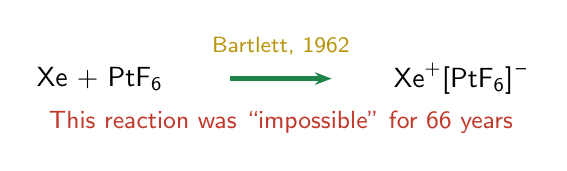
\begin{tikzpicture}[every node/.style={font=\sffamily\small}, scale=0.92]
  % Reaction arrow
  \node[font=\sffamily\normalsize] at (0,0) {\ce{Xe} + \ce{PtF6}};
  \draw[-{Stealth[length=6pt]}, ultra thick, ModuleColor]
    (1.8,0) -- (3.2,0);
  \node[font=\sffamily\normalsize] at (5.0,0)
    {\ce{Xe+[PtF6]-}};
  \node[font=\sffamily\footnotesize, text=DiscoveryColor]
    at (2.5,0.45) {Bartlett, 1962};
  \node[font=\sffamily\small, text=WarningColor]
    at (2.5,-0.6)
    {This reaction was ``impossible'' for 66 years};
\end{tikzpicture}
\end{center}

Bartlett mixed xenon and \ce{PtF6} gas in a flask.
An immediate orange-yellow solid formed.
The ``inert'' gas had been oxidised.

Within months, \ce{XeF2}, \ce{XeF4}, and \ce{XeF6}
were synthesised by other groups.
Xenon chemistry blossomed overnight.

\begin{center}
\small
\begin{tabular}{llll}
\toprule
Compound & Structure & Xe oxidation state & Stability \\
\midrule
\ce{XeF2}  & linear          & $+2$ & stable, white solid \\
\ce{XeF4}  & square planar   & $+4$ & stable, colourless \\
\ce{XeF6}  & distorted octahedral & $+6$ & reactive \\
\ce{XeO3}  & pyramidal       & $+6$ & explosive \\
\ce{XeO4}  & tetrahedral     & $+8$ & extremely unstable \\
\ce{XeOF4} & square pyramidal & $+6$ & stable \\
\bottomrule
\end{tabular}
\end{center}

The key: xenon's large size (lower IE) and the extreme
electronegativity of fluorine and oxygen make bond
formation energetically favourable for the heaviest
noble gases.
Helium, neon, and argon (high IE, small radius) still
form essentially no stable compounds.

\begin{discoverybox}
\textbf{Why Xe bonds and He doesn't: a quantitative comparison.}

For a noble gas to bond to fluorine, the energy of the
\ce{Ng-F} bond must overcome the energy cost of
``unpairing'' the noble gas's full shell.

A rough estimate: the energy barrier is proportional
to the ionisation energy (higher IE = more stable,
harder to disrupt).

\begin{center}
\small
\begin{tabular}{lccc}
\toprule
Noble gas & IE$_1$ (eV) & Forms fluoride? & Reason \\
\midrule
He  & 24.6 & No  & IE far too high \\
Ne  & 21.6 & No  & IE still very high \\
Ar  & 15.8 & Barely & \ce{ArF} transient \\
Kr  & 14.0 & Yes (KrF$_2$, unstable) & Marginal \\
Xe  & 12.1 & Yes (stable) & IE comparable to O$_2$ \\
Rn  & 10.7 & Yes (predicted) & Lower IE \\
\bottomrule
\end{tabular}
\end{center}

The periodic trend (IE decreases down the group)
directly explains why only the heavy noble gases
are chemically accessible.
\end{discoverybox}

\subsection{Noble Gases in the Modern World}

Despite their inertness, noble gases are chemically
and technologically essential.

\begin{itemize}[nosep, leftmargin=2em]
  \item \textbf{Helium} (from natural gas wells, produced
        by radioactive decay): MRI machines, cryogenics,
        pressurising rocket fuel, inflating weather balloons.
        It is genuinely irreplaceable for some cryogenic
        applications --- there is no substitute.
  \item \textbf{Argon} (from fractional distillation of air):
        inert atmosphere for welding and semiconductor
        manufacture, filling incandescent light bulbs
        to prevent filament oxidation.
  \item \textbf{Neon, krypton, xenon}: lighting, lasers
        (excimer lasers use ArF or KrF),
        anaesthesia (xenon is an anaesthetic),
        ion propulsion for spacecraft (xenon ions).
  \item \textbf{Radon}: a radiation hazard from natural
        uranium decay in rocks; monitored in buildings
        in granite-rich regions.
\end{itemize}

\begin{problembox}
\begin{enumerate}[label=\textbf{\arabic*.}]
  \item \textbf{Identifying argon from data.}
        Ramsay had an unknown gas.
        Its properties: density 1.784 g/L (STP),
        monatomic, colourless, unreactive,
        spectral lines at 750.4 nm, 696.5 nm, 706.7 nm.
        \begin{enumerate}[label=(\alph*)]
          \item Calculate its molar mass.
          \item Using Mendeleev's table ordered by mass,
                identify what period and group it must
                belong to (given that it is chemically inert).
          \item The element between Cl ($Z=17$) and K ($Z=19$)
                by mass would be expected to be between
                them in the table.
                Confirm that argon fits between the halogens
                and alkali metals in the modern table.
          \item Ramsay noticed the atomic mass of argon (39.9)
                is higher than potassium (39.1).
                Why must argon come \emph{before} potassium
                in the table despite being heavier?
        \end{enumerate}

  \item \textbf{Predicting noble gas compounds.}
        Krypton difluoride (\ce{KrF2}) is an unstable
        but real compound.
        \begin{enumerate}[label=(\alph*)]
          \item The \ce{Kr-F} bond dissociation energy
                is 50 kJ/mol.
                The \ce{F-F} bond energy is 157 kJ/mol
                and the IE of Kr is 14.0 eV.
                Use a Born-Haber type cycle to estimate
                whether \ce{KrF2} formation from the elements
                is exo- or endothermic.
          \item \ce{KrF2} decomposes slowly at room temperature
                but rapidly above \SI{60}{\degreeCelsius}.
                What does this tell you about the
                thermodynamics vs kinetics of its stability?
          \item Would you predict \ce{ArF2} to be more
                or less stable than \ce{KrF2}?
                Justify quantitatively using IE values.
        \end{enumerate}

  \item \textbf{VSEPR and xenon compounds.}
        Apply VSEPR theory to predict the geometry of:
        \begin{enumerate}[label=(\alph*)]
          \item \ce{XeF2} (Xe has 3 lone pairs + 2 bond pairs)
          \item \ce{XeF4} (Xe has 2 lone pairs + 4 bond pairs)
          \item \ce{XeF6} (Xe has 1 lone pair + 6 bond pairs)
          \item \ce{XeO3} (Xe has 1 lone pair + 3 double bonds)
        \end{enumerate}
        Draw the Lewis structure for each, showing lone pairs.
\end{enumerate}
\end{problembox}

\subsection*{Where the Inertness Model Breaks}

\begin{modelbreaks}
The ``noble gases are inert'' rule has exceptions beyond xenon:

\begin{itemize}[nosep, leftmargin=2em]
  \item \textbf{Clathrate compounds}: noble gases can be physically
        trapped inside cage-like crystal structures
        (e.g.\ \ce{Xe * 5.75 H2O}, xenon clathrate hydrate).
        No covalent bonds form, but the gas is chemically
        sequestered. This is not a true chemical compound,
        but the distinction is philosophically uncomfortable.
  \item \textbf{Van der Waals molecules}: \ce{ArHF},
        \ce{NeHF}, and similar weakly bound complexes
        are observed spectroscopically.
        They exist only at very low temperatures and
        are bound by $\sim 1$ kJ/mol.
        Are these ``compounds''?
  \item \textbf{Endohedral fullerenes}: noble gas atoms
        can be trapped inside \ce{C60} molecules
        (e.g.\ Ar@C$_{60}$).
        The notation ```@''' means ``inside.''
  \item \textbf{Oganesson (Z=118)}: the heaviest known noble gas.
        Relativistic calculations predict it may not be
        a gas at room temperature, may have significant
        electron affinity, and may form compounds more
        readily than xenon. The ``noble gas'' label
        may not apply at all to period-7 group-18 elements.
\end{itemize}
\end{modelbreaks}

\subsection*{Deep Problems}

\begin{deepbox}
\begin{enumerate}[label=\textbf{D\arabic*.}]

  \item \textbf{Bartlett's reasoning quantified.}

        Bartlett knew: IE(Xe) $= 12.13$ eV,
        IE(O$_2$) $= 12.07$ eV,
        and \ce{PtF6} had already been shown to oxidise O$_2$.

        \begin{enumerate}[label=(\alph*)]
          \item The reaction \ce{O2 + PtF6 -> O2+[PtF6]-}
                is observed to be exothermic.
                What does this tell you about the electron
                affinity of \ce{PtF6} relative to IE(O$_2$)?
          \item Using only the ionisation energy argument,
                construct a thermochemical cycle showing why
                Bartlett predicted \ce{Xe + PtF6 -> Xe+[PtF6]-}
                would also be exothermic.
          \item The actual product of Bartlett's reaction
                was later shown to be more complex
                (\ce{[XeF]+[PtF6]-} and related species).
                Does this invalidate the significance of
                his experiment?
          \item Why would an argument based purely on
                ionisation energies be expected to work here?
                What approximations does it make?
        \end{enumerate}

  \item \textbf{The noble gases and the Big Bang.}

        Helium is the second most abundant element in the
        universe (about 24\% by mass).
        Almost all of it was made in Big Bang nucleosynthesis
        (first 3 minutes after the Big Bang).

        \begin{enumerate}[label=(\alph*)]
          \item The Sun converts H to He via the p-p chain.
                The net reaction is:
                \[
                  4\,\ce{^1H} \to \ce{^4He} + 2e^+ + 2\nu_e + 2\gamma
                \]
                The mass deficit per reaction is $\Delta m = 4.8\times10^{-29}$ kg.
                Calculate the energy released per reaction
                in MeV, using $E = \Delta mc^2$.
          \item The Sun's luminosity is $3.85\times10^{26}$ W.
                How many kg of hydrogen does the Sun
                convert to helium per second?
          \item Earth's helium supply (trapped in geological
                formations) is finite and non-renewable
                on human timescales (helium escapes to space).
                Given that helium is essential for MRI machines
                and certain semiconductor processes,
                discuss the economics and policy implications
                of helium scarcity.
        \end{enumerate}

\end{enumerate}
\end{deepbox}

\subsection*{Reflection}

\begin{reflectionbox}
\begin{enumerate}[label=\textbf{R\arabic*.}]
  \item Chemistry textbooks stated for 66 years that noble
        gases form no compounds.
        This was consistent with all known evidence.
        \textbf{When is it appropriate to state a scientific
        claim as absolute rather than as a strong generalisation?}
        What is the cost of stating ``X never happens''
        versus ``X has never been observed to happen''?

  \item Bartlett's discovery depended on knowing IE(Xe) $\approx$ IE(O$_2$)
        and reasoning by analogy.
        \textbf{Is this a discovery or a prediction confirmed?}
        At what point does an experiment verify a prediction
        versus constitute an independent discovery?

  \item The noble gases were a complete surprise to the
        19th-century chemist.
        They had no valence, formed no bonds, sat outside
        all known chemical families.
        \textbf{Are there other ``impossible'' groups of elements
        or substances that current chemistry might be
        missing for analogous reasons?}
        How would we know?
\end{enumerate}
\end{reflectionbox}

\vspace{1.5em}
\begin{center}
\begin{tcolorbox}[enhanced, colback=DiscoveryColor!8, colframe=DiscoveryColor,
  width=0.88\textwidth, arc=3pt]
\centering\sffamily\small
\textbf{What we invented in this module.}\\[4pt]
We learned that the periodic table has a hidden group ---
one that Mendeleev had no room for in 1869 because no member
had yet been found.
The noble gases are the \emph{endpoints} of each period,
the fully-filled configurations that give the octet rule
its driving force.
Their discovery required the table's period lengths to expand
from 7 to 8.
Their chemistry --- zero for 66 years, then rich once the right
reagent was tried --- illustrates how a single experiment
can overturn a generation of certainty.
The lesson: ``has never been observed'' and ``cannot happen''
are very different claims.
\end{tcolorbox}
\end{center}

\vspace{2em}
\noindent\textcolor{JourneyColor!40}{\rule{\textwidth}{0.6pt}}
\begin{center}
\textit{\sffamily\small
Module 3.3 complete. Continue to Module 3.4:\\
\textbf{Transition Metals: The $d$-Block and Its Anomalies}.}
\end{center}

\end{document}